\newpage
\section{Permutations and combinations}
%%%%%%%%%%%%%%%%%%%%%%%%%%%%%%%%%%%%%%%%%%%%%
%%%%%%%%%%%%%%%%%%%%%%%%%%%%%%%%%%%%%%%%%%%%%
%%%%%%%%%%%%%%%%%%%%%%%%%%%%%%%%%%%%%%%%%%%%%
%%%%%%%%%%%%%%%%%%%%%%%%%%%%%%%%%%%%%%%%%%%%%
%% 1.1 Arrangements in a line %%%
%%%%%%%%%%%%%%%%%%%%%%%%%%%%%%%%%%%%%%%%%%%%%
%%%%%%%%%%%%%%%%%%%%%%%%%%%%%%%%%%%%%%%%%%%%%
%%%%%%%%%%%%%%%%%%%%%%%%%%%%%%%%%%%%%%%%%%%%%
%%%%%%%%%%%%%%%%%%%%%%%%%%%%%%%%%%%%%%%%%%%%%
\subsection{Arrangements in a line}

\begin{itemize}
	\setlength\itemsep{0.5em}
	\item Arrangements of \textbf{distinct} items	
	
	The number of different arrangements of $n$ distinct items is 
	\[
	n \times (n-1) \times (n-2) \times \ldots \times 3 \times 2 \times 1 = n!	\]
	\item Arrangements when items are \textbf{not} distinct
	
	The number of different arrangements of $n$ items of which $p$ of one type are alike, $q$ of another type are alike, $r$ of another type are alike, and so on, is 
	\[
	\frac{n!}{p!\times q! \times r!\times \ldots}.
	\]
	\item Arrangements when there are restrictions
	\begin{itemize}
			\setlength\itemsep{0.5em}
		\item particular items have to be together, or must be separated.
		\item not all $\&$ all not.
	\end{itemize}
	
	\item Arrangemnets when \textbf{repetitions} are allowed
\end{itemize}

\exercise   %%%%%%%% Exercise 9

\begin{enumerate}
	\item Each of the letters of the word \textbf{CAMBRIDGE} is written on a card and the cards are placed in a line.
	\begin{enumerate}
		\item How many different arrangements are there?
		\item How many arrangements begin with \textbf{CAM}.
	\end{enumerate}

  \item Find the number of different arrangements using all ten letters of the word \textbf{STATISTICS}.
  
  
  \item The word \textbf{ARGENTINA} includes the four consonants \textbf{R}, \textbf{G}, \textbf{N}, \textbf{T} and the three vowels \textbf{A}, \textbf{E},  \textbf{I}.
  \begin{enumerate}
  	\item Find the number of different arrangements using all nine letters.
  	\item How many of these arrangements have a consonant at the beginning, then a vowel, then another consonant, and so on alternately? 
  \end{enumerate}

\item Issam has $11$ different CDs, of which $6$ are pop music, $3$ are jazz and $2$ are classical.
How many different arrangements of all $11$ CDs on a shelf are there if the jazz CDs are all next to each other.

\item The eight sopranos in a choir are asked to stand in a line, but Ruby and Grace refuse to stand next to each other. How many different arrangements can there be?

\item How many $5$-digit \textbf{odd} numbers can be made with the digits $2$, $3$, $6$, $7$, $8$

\begin{enumerate}
	\item if repetitions are not allowed, for example, $63\,287$.
	\item if repetitions are allowed, for example, $88\,663$.
\end{enumerate}


\item  \begin{enumerate}
	\item Safebank requires its customers to use a four-digit PIN to access their account. Customers can choose any set of $4$ digits from $0$, $1$, $2$, $\ldots$, 9 and digits may be repeated. How many possible four-digit PINs are there?
	\item Smartbank requires its customers to use a password consisting of four lower-case letters. Repetitions are allowed. How many  possible passwords are there?
	\item Excelbank requires its customers to use a pass-code consisting of four letters followed by four digits. Repititions are allowed. How many possible pass-codes are there?
\end{enumerate}

\end{enumerate}



\exercise   %%%% -- Exercise 10

\begin{enumerate}
	\item Find the number of ways to arrange the letters of each of the following words:
	\begin{enumerate}
		\item SPIDER
		\item SANDWICH
		\item PENGUIN
		\item BLACKBERRY
		\item MATHEMATICAL
	\end{enumerate}

   \item Find the number of ways in which all eight letters of the word \textbf{ADVANCED} can be arranged if the arrangement must begin and end with an \textbf{A}.
   
   \item Find the number of ways in which all eight letters of the word \textbf{NEEDLESS} can be arranged:
   \begin{enumerate}
   	\item if there are no restrictions,
   	\item if the arrangement must end with \textbf{N},
   	\item if the three letters \textbf{E} must be placed next to each other,
   	\item if the two letters \textbf{S} must  not be placed next to each other,
   	\item if the three letters \textbf{E} must be placed together and the letter \textbf{S} must not be place together.
   \end{enumerate}

\item Five boys and four girls sit on a bench. In how many ways can they be seated if no two boys  sit next to each other?

\item Three identical yellow ballons, two identical red ballons and two identical blue ballons are strung in a row to celebrate Shema's birthday. Calculate the number of arrangements if:

\begin{enumerate}
	\item the ballon at each end is the same colour,
	\item the yellow ballons are next to each other and the blue ballons are not next to each other.
\end{enumerate}

\item Find how many arrangements there are of the nine letters in the word \textbf{GOLD\,MEDAL}

\begin{enumerate}
	\item if there are no restrictions in the order of the letters,
	\item if the two letters \textbf{D} come first and the two letters \textbf{L} come last.
\end{enumerate}


\item Four identical tins of peaches and six identical tins of pears are arranged in a row on a shelf. Calculate the number of different arrangements if the tin at eache end contains the same type of fruit.

\item Three girls and seven boys stand in a line. Calculate the number of different arrangements if:
\begin{enumerate}
	\item the two youngest pupils are separated,
	\item all three girls stand together.
\end{enumerate}

\item There are 10 seats in a row in a theatre. In how many ways can $5$ couples be seated in a row if each couple sits together?

\item Find how many different arrangements there are of eleven letters of the word \textbf{PROBABILITY} if the two letters \textbf{B} are at the beginning and the two letters \textbf{I} are at the end.

\item \boxed{1} \, \boxed{3} \, \boxed{3} \, \boxed{8} \, \boxed{8} \, \boxed{8}

The above cards are placed in a line to form a $6$-digit number. How many numbers can be made:
\begin{enumerate}
	\item if there are no restrictions,
	\item if the number ends in $3$,
	\item if the number is odd?
\end{enumerate}

\end{enumerate}
\newpage
%%%%%%%%%%%%%%%%%%%%%%%%%%%%%%%%%%%%%%%%%%%%%
%%%%%%%%%%%%%%%%%%%%%%%%%%%%%%%%%%%%%%%%%%%%%
%%%%%%%%%%%%%%%%%%%%%%%%%%%%%%%%%%%%%%%%%%%%%
%%%%%%%%%%%%%%%%%%%%%%%%%%%%%%%%%%%%%%%%%%%%%
%% 1.2 Permuations of $r$ items from $n$ items %%%
%%%%%%%%%%%%%%%%%%%%%%%%%%%%%%%%%%%%%%%%%%%%%
%%%%%%%%%%%%%%%%%%%%%%%%%%%%%%%%%%%%%%%%%%%%%
%%%%%%%%%%%%%%%%%%%%%%%%%%%%%%%%%%%%%%%%%%%%%
%%%%%%%%%%%%%%%%%%%%%%%%%%%%%%%%%%%%%%%%%%%%%
\subsection{Permuations of $r$ items from $n$ items}

Suppose $A$, $B$, $C$, $D$, $E$, $F$, $G$ are put into $4$ spaces,
\medskip

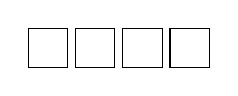
\begin{tikzpicture}
	\draw (-0.25,-0.25) rectangle (0.25,0.25);
	\draw (0.35,-0.25) rectangle (0.85,0.25);
	\draw (0.95,-0.25) rectangle (1.45,0.25);
	\draw (1.55,-0.25) rectangle (2.05,0.25);
\end{tikzpicture}

\medskip

number of ways of arrangements will be $7\times 6 \times 5 \times 4$, which is also denoted by $_{7}\text{P}_4$. Notice that 
\[
7\times 6 \times 5 \times 4=\frac{7\times 6 \times 5 \times 4 \times 3 \times 2 \times 1}{3 \times 2 \times 1} = \frac{7!}{3!} = \frac{7!}{(7-4)!}
\]

In general, the number of permutations, of $r$ items taken from $n$ \textbf{distinct} item is 
\[
_{n}\text{P}_r = \frac{n!}{(n-r)!}.
\]

Special case, $0! =1$.

\medskip

\textbf{Restrictions:}

\begin{itemize}
	\setlength\itemsep{2.5em}
	\item  Not distinct.
	\item  Together.
	\item  others.
	
\end{itemize}

\bigskip

Challenge:  $8$ students sit on $12$ chairs in a row. Among these eight students, $A$ and $B$ must be together. Find the number of different arrangements.

\bigskip

\bigskip

\bigskip

\exercise  %%% Exercise 11
 
\begin{enumerate}
	\item Find how many numbers bigger than $30\,000$ but smaller than $40\,000$ can be formed the digits $2,3,4,5,6,7,8$ if no digit is repeated and the number must be a multiple of $5$. 
	
	\item A security code cosists of $4$ letters chosen from $A$, $B$, $C$, $D$, $E$, $F$, $G$  followed by $3$ digits chosen from $0$, $1$, $2$, $3$, $4$, $5$.
	
	Examples are $BCDG102$ (without repetitions) and $CCDD225$ (with repetitions).
	
	Show that more than five times as many codes can be made when repetitions are allowed than when repetitions are not allowed.
	
	
	\item  Rory is playing a game in which he has to place coloured pegs into holes in a board. He has $6$ identical red pegs and the board has $10$ holes. How many different arrangements are there for placing $6$ pegs and leaving $4$ empty holes?  
	
	\item If repetitions are not allowed, how many numbers can be formed with the digits $3$, $4$, $5$, $6$ $7$ 
	\begin{enumerate}
		\item using three of the digits,
		\item using one or more of the digits? 
	\end{enumerate}


  \item  There are $10$ seats in the front row at a theatre. Six people are shown to this row. In how many different ways can they be seated if 
  \begin{enumerate}
  	\item there are no restrictions,
  	\item two particular people in the group must sit next to each other?
  \end{enumerate}
	
\end{enumerate}


\newpage
%%%%%%%%%%%%%%%%%%%%%%%%%%%%%%%%%%%%%%%%%%%%%
%%%%%%%%%%%%%%%%%%%%%%%%%%%%%%%%%%%%%%%%%%%%%
%%%%%%%%%%%%%%%%%%%%%%%%%%%%%%%%%%%%%%%%%%%%%
%%%%%%%%%%%%%%%%%%%%%%%%%%%%%%%%%%%%%%%%%%%%%
%% 1.2 Combinations of $r$ items from $n$ items %%%
%%%%%%%%%%%%%%%%%%%%%%%%%%%%%%%%%%%%%%%%%%%%%
%%%%%%%%%%%%%%%%%%%%%%%%%%%%%%%%%%%%%%%%%%%%%
%%%%%%%%%%%%%%%%%%%%%%%%%%%%%%%%%%%%%%%%%%%%%
%%%%%%%%%%%%%%%%%%%%%%%%%%%%%%%%%%%%%%%%%%%%%
\subsection{Combinations of $r$ items from $n$ items}

A combination is a selection of some items where the order of the selected item $\underline{\hspace{4cm}}$.

\medskip

In general, the number of combinations of $r$ items from $n$ \textbf{distinct} items is given by

\[
 \binom{n}{r}  =        \, _{n}\text{C}_r       =     \frac{n!}{r!(n-r)!}. 
\]

Notice, "\textbf{distinct}" is a very important conditions for combinations.
\medskip

What happens when the selections are from items that are \textbf{NOT} distinct?

\medskip

For example: Three letters are selected at random from the letters of the word \textbf{BIOLOGY}. Find the total number of selections.

\bigskip

\bigskip

 


\exercise  %%  Exercise 12

\begin{enumerate}
	\item A team of $3$ is to be chosen from $10$ athletes. How many different teams could be chosen?
	
	\item  Without using a calculator, evaluate $\displaystyle \binom{12}{9}$ and $\displaystyle \binom{12}{3}$.
	
	
	\item  Issam has $11$ different CDs of which $6$ are pop music, $3$ are jazz and $2$ are classical. Issam makes a selection of $2$ pop music CDs, $2$ jazz CDs are $1$ classical CD.
	
	
	How many different possible selections can be made?
	
	
	\item A collection of $18$ books contain one Harry Potter book. Linda is going to choose $6$ of these books to take on holiday.
	
	\begin{enumerate}
		\item In how many ways can she choose $6$ books?
		\item How many of these choices will include the Harry Potter book?
	\end{enumerate}


\item  A committee of $5$ people is to be chosen from $6$ men and $4$ women. In how many ways can this be done:

\begin{enumerate}
	\item if there must be $3$ men and $2$  women on the committee,
	\item if there must be more than men than women on the committee,
	\item if there must be $3$ men and $2$ women, and one particular woman refuses to be on the committee with one particular man?
\end{enumerate}


\item In a mixed pack of coloured light bulbs there are three red bulbs, one yellow bulbs, one blue bulbs and one green bulbs. Four bulbs are selected at random from the pack. How many different selections are possible?
	
	
\item  Four letters are to be selected from the letters in the word $RIGIDITY$. How many different combinations are there?	


\item The letters of the word $POSSESSES$ are written on nine cards, one on each card. The cards are shuffled and four of them are selected and arranged in a straight line.
\begin{enumerate}
	\item How many possible selections are there of four letters?
	\item How many arrangments are there of four letters?
\end{enumerate}
\end{enumerate}	
	
\newpage 


	
\mis   %%%%%%%%%  --  miscellaneous 2

%%%%%%%%%%%%%%%%%%%%%%%%
%%%%%%%%%%%%%%%%%%%%%%%%
%%% Q1 m17_qp_62_5 %%%%%
%%%%%%%%%%%%%%%%%%%%%%%%
%%%%%%%%%%%%%%%%%%%%%%%%
%%%%%%%%%%%%%%%%%%%%%%%%
\begin{enumerate}
	\item \begin{enumerate}
		\item A plate of cakes holds $12$ different cakes. Find the number of ways these cakes can be shared between Alex and James if each receives an odd number of cakes. \hfill [3]
		\item Another plate holds $7$ cup cakes, each with a different colour icing, and $4$ brownies, each of a different size. Find the number of different ways these $11$ cakes can be arranged in a row if no	brownie is next to another brownie. \hfill [3]
		\item  A plate of biscuits holds $4$ identical chocolate biscuits, $6$ identical shortbread biscuits and $2$ identical gingerbread biscuits. These biscuits are all placed in a row. Find how many different	arrangements are possible if the chocolate biscuits are all kept together. \hfill [3]
		
			\end{enumerate}
%%%%%%%%%%%%%%%%%%%%%%%%
%%%%%%%%%%%%%%%%%%%%%%%%
%%% Q2 m18_qp_62_2 %%%%%
%%%%%%%%%%%%%%%%%%%%%%%%
%%%%%%%%%%%%%%%%%%%%%%%%
%%%%%%%%%%%%%%%%%%%%%%%%		
		
	\item A selection of $3$ letters from the $8$ letters of the word \textbf{COLLIDER} is made.
	
	\begin{enumerate}
		\item How many different selections of $3$ letters can be made if there is exactly one \textbf{L}? \hfill[1]
		\item How many different selections of $3$ letters can be made if there are no restrictions? \hfill [3]
	\end{enumerate}
		
		
%%%%%%%%%%%%%%%%%%%%%%%%
%%%%%%%%%%%%%%%%%%%%%%%%
%%% Q3 m19_qp_62_7 %%%%%
%%%%%%%%%%%%%%%%%%%%%%%%
%%%%%%%%%%%%%%%%%%%%%%%%
%%%%%%%%%%%%%%%%%%%%%%%%		
		
	\item Find the number of different arrangements that can bemade of all $9$ letters in the word \textbf{CAMERAMAN} in each of the following cases.	
	
  \begin{enumerate}
  	\item There are no restrictions. \hfill[2]
  	\item The \textbf{A}s occupy the $1$st, $5$th and $9$th positions. \hfill[1]
  	\item  There is exactly one letter between the \textbf{M}s. \hfill [4]
  \end{enumerate}
		
		
		
%%%%%%%%%%%%%%%%%%%%%%%%
%%%%%%%%%%%%%%%%%%%%%%%%
%%% Q4 s17_qp_61_7 %%%%%
%%%%%%%%%%%%%%%%%%%%%%%%
%%%%%%%%%%%%%%%%%%%%%%%%
%%%%%%%%%%%%%%%%%%%%%%%%	

\item  \begin{enumerate}
	\item Eight children of different ages stand in a random order in a line. Find the number of different ways this can be done if none of the three youngest children stand next to each other. \hfill[3]
	\item David chooses $5$ chocolates from $6$ different dark chocolates, $4$ different white chocolates and $1$ milk chocolate. He must choose at least one of each type. Find the number of different selections he can make. \hfill[4]
	\item A password for Chelsea’s computer consists of $4$ characters in a particular order. The characters are chosen from the following.
	\begin{itemize}
		\setlength\itemsep{0.5em}
		\item The $26$ capital letters A to Z
		\item The $9$ digits $1$ to $9$
		\item The $5$ symbols $\#$ $\sim$  $*$  $?$  $!$
	\end{itemize} 
	The password must include at least one capital letter, at least one digit and at least one symbol.	No character can be repeated. Find the number of different passwords that Chelsea can make. \hfill 	[4]
\end{enumerate}	
		
%%%%%%%%%%%%%%%%%%%%%%%%
%%%%%%%%%%%%%%%%%%%%%%%%
%%% Q5 s17_qp_62_6 %%%%%
%%%%%%%%%%%%%%%%%%%%%%%%
%%%%%%%%%%%%%%%%%%%%%%%%
%%%%%%%%%%%%%%%%%%%%%%%%	

\item A library contains $4$ identical copies of book A, $2$ identical copies of book B and $5$ identical copies of book C. These $11$ books are arranged on a shelf in the library.

\begin{enumerate}
	\item Calculate the number of different arrangements if the end books are either both book A or both book B. \hfill[4]
	\item Calculate the number of different arrangements if all the books A are next to each other and none of the books B are next to each other. \hfill [5]
\end{enumerate}
	
		
%%%%%%%%%%%%%%%%%%%%%%%%
%%%%%%%%%%%%%%%%%%%%%%%%
%%% Q6 s17_qp_63_6 %%%%%
%%%%%%%%%%%%%%%%%%%%%%%%
%%%%%%%%%%%%%%%%%%%%%%%%
%%%%%%%%%%%%%%%%%%%%%%%%

\item  \begin{enumerate}
	\item Find how many numbers between $3000$ and $5000$ can be formed from the digits $1$, $2$, $3$, $4$ and $5$,
	\begin{enumerate}
		\item if digits are not repeated, \hfill[2] 
		\item if digits can be repeated and the number formed is odd. \hfill[3]
	\end{enumerate}
\item A box of $20$ biscuits contains $4$ different chocolate biscuits, $2$ different oatmeal biscuits and $14$ different ginger biscuits. $6$ biscuits are selected from the box at random.

\begin{enumerate}
	\item Find the number of different selections that include the $2$ oatmeal biscuits. \hfill[2]
	\item Find the probability that fewer than $3$ chocolate biscuits are selected. \hfill[4]
\end{enumerate}

\end{enumerate}		






\end{enumerate}	
	
	
	
	\newpage 
	
	\exam   %%%%  Exam 2
	
	
\begin{enumerate}
	
%%%%%%%%%%%%%%%%%%%%%%%%
%%%%%%%%%%%%%%%%%%%%%%%%
%%% Q1 s18_qp_61_7 %%%%%
%%%%%%%%%%%%%%%%%%%%%%%%
%%%%%%%%%%%%%%%%%%%%%%%%
%%%%%%%%%%%%%%%%%%%%%%%%	
	
	\item Find the number of different ways in which all $9$ letters of the word \textbf{MINCEMEAT} can be arranged in	each of the following cases. 
	\begin{enumerate}[label=(\roman*)]
		\item There are no restrictions.  \hfill[1]
		\item No vowel (\textbf{A}, \textbf{E}, \textbf{I} are vowels) is next to another vowel. \hfill[4]
	\end{enumerate}
    $5$ of the $9$ letters of the word \textbf{MINCEMEAT} are selected.
    \begin{enumerate}[resume,label=(\roman*)]
    	\item Find the number of possible selections which contain exactly $1$ \textbf{M} and exactly $1$ \textbf{E}. \hfill[2]
    	\item  Find the number of possible selections which contain at least $1$ \textbf{M} and at least $1$ \textbf{E}. \hfill[3]
    \end{enumerate}


   
%%%%%%%%%%%%%%%%%%%%%%%%
%%%%%%%%%%%%%%%%%%%%%%%%
%%% Q2 s18_qp_62_6 %%%%%
%%%%%%%%%%%%%%%%%%%%%%%%
%%%%%%%%%%%%%%%%%%%%%%%%
%%%%%%%%%%%%%%%%%%%%%%%%

\item  \begin{enumerate}[label=(\roman*)]
	\item Find the number of ways in which all $9$ letters of the word \textbf{AUSTRALIA} can be arranged in each of the following cases.
	
	\begin{enumerate}[label=(\alph*)]
		\item All the vowels (\textbf{A}, \textbf{I}, \textbf{U} are vowels) are together. \hfill [3]
		\item The letter \textbf{T} is in the central position and each end position is occupied by one of the other consonants (\textbf{R}, \textbf{S}, \textbf{L}). \hfill [3]
	\end{enumerate}
\item Donna has $2$ necklaces, $8$ rings and $4$ bracelets, all different. She chooses $4$ pieces of jewellery.

How many possible selections can she make if she chooses at least $1$ necklace and at least $1$
bracelet?  \hfill [4]
\end{enumerate}


%%%%%%%%%%%%%%%%%%%%%%%%
%%%%%%%%%%%%%%%%%%%%%%%%
%%% Q3 s18_qp_63_7 %%%%%
%%%%%%%%%%%%%%%%%%%%%%%%
%%%%%%%%%%%%%%%%%%%%%%%%
%%%%%%%%%%%%%%%%%%%%%%%%

\item Find the number of ways the $9$ letters of the word \textbf{SEVENTEEN} can be arranged in each of the following cases.

\begin{enumerate}[label=(\roman*)]
	\item One of the letter \textbf{E}s is in the centre with $4$ letters on either side. \hfill[2]
	\item No \textbf{E} is next to another \textbf{E}. \hfill[3]
\end{enumerate}
$5$ letters are chosen from the $9$ letters of the word \textbf{SEVENTEEN}.
\begin{enumerate}[resume,label=(\roman*)]
	\item Find the number of possible selections which contain exactly $2$ \textbf{E}s and exactly 2 \textbf{N}s. \hfill[1]
	\item Find the number of possible selections which contain at least $2$ \textbf{E}s. \hfill[4]
\end{enumerate}

%%%%%%%%%%%%%%%%%%%%%%%%
%%%%%%%%%%%%%%%%%%%%%%%%
%%% Q4 s19_qp_61_7 %%%%%
%%%%%%%%%%%%%%%%%%%%%%%%
%%%%%%%%%%%%%%%%%%%%%%%%
%%%%%%%%%%%%%%%%%%%%%%%%

\item  Freddie has $6$ toy cars and $3$ toy buses, all different. He chooses $4$ toys to take on holiday with him.

\begin{enumerate}[label=(\roman*)]
	\item In how many different ways can Freddie choose $4$ toys? \hfill[1]
	\item How many of these choices will include both his favourite car and his favourite bus? \hfill[2]
\end{enumerate}

Freddie arranges these $9$ toys in a line.

\begin{enumerate}[resume,label=(\roman*)]
	\item Find the number of possible arrangements if the buses are all next to each other. \hfill[3]
	\item  Find the number of possible arrangements if there is a car at each end of the line and no buses are next to each other. \hfill[3]
\end{enumerate}


%%%%%%%%%%%%%%%%%%%%%%%%
%%%%%%%%%%%%%%%%%%%%%%%%
%%% Q5 s19_qp_62_7 %%%%%
%%%%%%%%%%%%%%%%%%%%%%%%
%%%%%%%%%%%%%%%%%%%%%%%%
%%%%%%%%%%%%%%%%%%%%%%%%

\item  \begin{enumerate}[label=(\roman*)]
	\item A group of $6$ teenagers go boating. There are three boats available. One boat has room for $3$ people, one has room for $2$ people and one has room for $1$ person. Find the number of different ways the group of 6 teenagers can be divided between the three boats.\hfill [3]
	\item Find the number of different $7$-digit numbers which can be formed from the seven digits $2$, $2$, $3$, $7$, $7$, $7$, $8$ in each of the following cases.
	\begin{enumerate}[label=(\alph*)]
		\item The odd digits are together and the even digits are together. \hfill [3]
		\item The $2$s are not together. \hfill[4]
	\end{enumerate}
\end{enumerate}


%%%%%%%%%%%%%%%%%%%%%%%%
%%%%%%%%%%%%%%%%%%%%%%%%
%%% Q6 s19_qp_63_7 %%%%%
%%%%%%%%%%%%%%%%%%%%%%%%
%%%%%%%%%%%%%%%%%%%%%%%%
%%%%%%%%%%%%%%%%%%%%%%%%

\item  \begin{enumerate}[label=(\roman*)]
	\item Find the number of ways a committee of $6$ people can be chosen from $8$ men and $4$ women if there must be at least twice as many men as there are women on the committee. \hfill[3]
	\item Find the number of ways a committee of $6$ people can be chosen from $8$ men and $4$ women if $2$ particular men refuse to be on the committee together. \hfill[3]

\end{enumerate}
%%%%%%%%%%%%%%%%%%%%%%%%
%%%%%%%%%%%%%%%%%%%%%%%%
%%% Q7 w17_qp_61_6 %%%%%
%%%%%%%%%%%%%%%%%%%%%%%%
%%%%%%%%%%%%%%%%%%%%%%%%
%%%%%%%%%%%%%%%%%%%%%%%%


\item \begin{enumerate}[label=(\roman*)]
	\item A village hall has seats for $40$ people, consisting of $8$ rows with $5$ seats in each row. Mary,Ahmad, Wayne, Elsie and John are the first to arrive in the village hall and no seats are taken
	before they arrive.
	
	\begin{enumerate}[label=(\alph*)]
		\item How many possible arrangements are there of seatingMary, Ahmad,Wayne, Elsie and John
		assuming there are no restrictions? \hfill[2]
		\item How many possible arrangements are there of seatingMary, Ahmad,Wayne, Elsie and John
		if Mary and Ahmad sit together in the front row and the other three sit together in one of
		the other rows? \hfill[4]
	\end{enumerate}
\item  In how many ways can a team of $4$ people be chosen from 10 people if $2$ of the people, Ross and Lionel, refuse to be in the team together? \hfill [4]
\end{enumerate}



%%%%%%%%%%%%%%%%%%%%%%%%
%%%%%%%%%%%%%%%%%%%%%%%%
%%% Q8 w17_qp_62_6 %%%%%
%%%%%%%%%%%%%%%%%%%%%%%%
%%%%%%%%%%%%%%%%%%%%%%%%
%%%%%%%%%%%%%%%%%%%%%%%%

\item  \begin{enumerate}[label=(\roman*)]
	\item Find the number of different $3$-digit numbers greater than 300 that can be made from the digits $1$, $2$, $3$, $4$, $6$, $8$ if
\begin{enumerate}[label=(\alph*)]
	\item no digit can be repeated, \hfill[3]
	\item a digit can be repeated and the number made is even. \hfill[3]
\end{enumerate}
\item  A team of $5$ is chosen from $6$ boys and $4$ girls. Find the number of ways the team can be chosen if 
\begin{enumerate}[label=(\alph*)]
	\item there are no restrictions, \hfill[1]
	\item the team contains more boys than girls. \hfill[3]
\end{enumerate}
\end{enumerate}



%%%%%%%%%%%%%%%%%%%%%%%%
%%%%%%%%%%%%%%%%%%%%%%%%
%%% Q9 w17_qp_63_6 %%%%%
%%%%%%%%%%%%%%%%%%%%%%%%
%%%%%%%%%%%%%%%%%%%%%%%%
%%%%%%%%%%%%%%%%%%%%%%%%


\item  A car park has spaces for $18$ cars, arranged in a line. On one day there are $5$ cars, of different makes, parked in randomly chosen positions and $13$ empty spaces.

\begin{enumerate}[label=(\roman*)]
	\item Find the number of possible arrangements of the $5$ cars in the car park. \hfill[2]
	\item Find the probability that the $5$ cars are not all next to each other. \hfill[5]
\end{enumerate}
On another day, $12$ cars of different makes are parked in the car park. $5$ of these cars are red, $4$ are white and $3$ are black. Elizabeth selects $3$ of these cars.
\begin{enumerate}[resume,label=(\roman*)]
	\item Find the number of selections Elizabeth can make that include cars of at least $2$ different colours. 
	
	
	\quad \hfill	[5]
\end{enumerate}



%%%%%%%%%%%%%%%%%%%%%%%%
%%%%%%%%%%%%%%%%%%%%%%%%
%%% Q10 w18_qp_61_1 %%%%%
%%%%%%%%%%%%%%%%%%%%%%%%
%%%%%%%%%%%%%%%%%%%%%%%%
%%%%%%%%%%%%%%%%%%%%%%%%

\item  $9$ people are to be divided into a group of $4$, a group of $3$ and a group of $2$. In how many different ways can this be done? \hfill[3]


%%%%%%%%%%%%%%%%%%%%%%%%
%%%%%%%%%%%%%%%%%%%%%%%%
%%% Q11 w18_qp_61_3 %%%%%
%%%%%%%%%%%%%%%%%%%%%%%%
%%%%%%%%%%%%%%%%%%%%%%%%
%%%%%%%%%%%%%%%%%%%%%%%%

\item  In an orchestra, there are $11$ violinists, $5$ cellists and $4$ double bass players. A small group of $6$ musicians is to be selected from these $20$.

\begin{enumerate}[label=(\roman*)]
	\item How many different selections of $6$ musicians can be made if there must be at least $4$ violinists,	at least $1$ cellist and no more than $1$ double bass player? \hfill[4]
\end{enumerate}

The small group that is selected contains $4$ violinists, $1$ cellist and $1$ double bass player. They sit in a line to perform a concert.

\begin{enumerate}[resume,label=(\roman*)]
	\item How many different arrangements are there of these 6musicians if the violinistsmust sit together?
	
	\quad  \hfill	[3]
\end{enumerate}


%%%%%%%%%%%%%%%%%%%%%%%%
%%%%%%%%%%%%%%%%%%%%%%%%
%%% Q12 w18_qp_62_1 %%%%%
%%%%%%%%%%%%%%%%%%%%%%%%
%%%%%%%%%%%%%%%%%%%%%%%%
%%%%%%%%%%%%%%%%%%%%%%%%

\item  \begin{enumerate}[label=(\roman*)]
	\item How many different arrangements are there of the $11$ letters in the word \textbf{MISSISSIPPI}? \hfill[2]
	\item Two letters are chosen at random from the $11$ letters in the word \textbf{MISSISSIPPI}. Find the probability that these two letters are the same. \hfill[3]
\end{enumerate}



%%%%%%%%%%%%%%%%%%%%%%%%
%%%%%%%%%%%%%%%%%%%%%%%%
%%% Q13 w18_qp_62_4 %%%%%
%%%%%%%%%%%%%%%%%%%%%%%%
%%%%%%%%%%%%%%%%%%%%%%%%
%%%%%%%%%%%%%%%%%%%%%%%%

\item  \begin{enumerate}[label=(\roman*)]
	\item  Find the number of different ways that $5$ boys and $6$ girls can stand in a row if all the boys stand together and all the girls stand together. \hfill[3]
	\item Find the number of different ways that $5$ boys and $6$ girls can stand in a row if no boy stands next	to another boy. \hfill[3]
\end{enumerate} 


%%%%%%%%%%%%%%%%%%%%%%%%
%%%%%%%%%%%%%%%%%%%%%%%%
%%% Q14 w18_qp_63_1 %%%%%
%%%%%%%%%%%%%%%%%%%%%%%%
%%%%%%%%%%%%%%%%%%%%%%%%
%%%%%%%%%%%%%%%%%%%%%%%%

\item A group consists of $5$ men and $2$ women. Find the number of different ways that the group can stand in a line if the women are not next to each other. \hfill[3]


%%%%%%%%%%%%%%%%%%%%%%%%
%%%%%%%%%%%%%%%%%%%%%%%%
%%% Q15 w18_qp_63_4 %%%%%
%%%%%%%%%%%%%%%%%%%%%%%%
%%%%%%%%%%%%%%%%%%%%%%%%
%%%%%%%%%%%%%%%%%%%%%%%%
\item  Out of a class of $8$ boys and $4$ girls, a group of $7$ people is chosen at random.

\begin{enumerate}[label=(\roman*)]
	\item Find the probability that the group of $7$ includes one particular boy. \hfill[3]
	\item Find the probability that the group of $7$ includes at least $2$ girls. \hfill [4]
\end{enumerate}




%%%%%%%%%%%%%%%%%%%%%%%%
%%%%%%%%%%%%%%%%%%%%%%%%
%%% Q16 w19_qp_61_6 %%%%%
%%%%%%%%%%%%%%%%%%%%%%%%
%%%%%%%%%%%%%%%%%%%%%%%%
%%%%%%%%%%%%%%%%%%%%%%%%


\item  \begin{enumerate}[label=(\roman*)]
	\item Find the number of different ways in which all $12$ letters of the word \textbf{STEEPLECHASE} can be arranged so that all four \textbf{E}s are together. \hfill[1]
	\item Find the number of different ways in which all $12$ letters of the word \textbf{STEEPLECHASE} can be arranged so that the \textbf{S}s are not next to each other. \hfill [4]
\end{enumerate}
	Four letters are selected from the $12$ letters of the word \textbf{STEEPLECHASE}.
	\begin{enumerate}[resume,label=(\roman*)]
		\item Find the number of different selections if the four letters include exactly one \textbf{S}. \hfill[4]
	\end{enumerate}


%%%%%%%%%%%%%%%%%%%%%%%%
%%%%%%%%%%%%%%%%%%%%%%%%
%%% Q17 w19_qp_62_6 %%%%%
%%%%%%%%%%%%%%%%%%%%%%%%
%%%%%%%%%%%%%%%%%%%%%%%%
%%%%%%%%%%%%%%%%%%%%%%%%

\item  \begin{enumerate}[label=(\roman*)]
	\item Find the number of different ways in which the $9$ letters of the word \textbf{TOADSTOOL} can be	arranged so that all three \textbf{O}s are together and both \textbf{T}s are together. \hfill[1]
	\item Find the number of different ways in which the $9$ letters of the word \textbf{TOADSTOOL} can be arranged so that the \textbf{T}s are not together. \hfill[4]
	\item  Find the probability that a randomly chosen arrangement of the $9$ letters of the word \textbf{TOADSTOOL}	has a \textbf{T} at the beginning and a \textbf{T} at the end. \hfill[2]
	\item Five letters are selected fromthe $9$ letters of the word \textbf{TOADSTOOL}. Find the number of different selections if the five letters include at least $2$ \textbf{O}s and at least $1$ \textbf{T}. \hfill[4]
\end{enumerate}


%%%%%%%%%%%%%%%%%%%%%%%%
%%%%%%%%%%%%%%%%%%%%%%%%
%%% Q18 w19_qp_63_2 %%%%%
%%%%%%%%%%%%%%%%%%%%%%%%
%%%%%%%%%%%%%%%%%%%%%%%%
%%%%%%%%%%%%%%%%%%%%%%%%


\item  \begin{enumerate}[label=(\roman*)]
	\item How many different arrangements are there of the $9$ letters in the word \textbf{CORRIDORS}? \hfill[2]
	\item  How many different arrangements are there of the $9$ letters in the word \textbf{CORRIDORS} in which
	the first letter is \textbf{D} and the last letter is \textbf{R} or \textbf{O}? \hfill [3]
\end{enumerate}


%%%%%%%%%%%%%%%%%%%%%%%%
%%%%%%%%%%%%%%%%%%%%%%%%
%%% Q18 w19_qp_63_3 %%%%%
%%%%%%%%%%%%%%%%%%%%%%%%
%%%%%%%%%%%%%%%%%%%%%%%%
%%%%%%%%%%%%%%%%%%%%%%%%

\item  A sports team of $7$ people is to be chosen from $6$ attackers, $5$ defenders and $4$ midfielders. The team must include at least $3$ attackers, at least $2$ defenders and at least $1$ midfielder.

\begin{enumerate}[label=(\roman*)]
	\item In how many different ways can the team of $7$ people be chosen? \hfill[4]
\end{enumerate}

The team of $7$ that is chosen travels to a match in two cars. A group of $4$ travel in one car and a group of $3$ travel in the other car.

\begin{enumerate}[resume,label=(\roman*)]
	\item In how many different ways can the team of $7$ be divided into a group of $4$ and a group of $3$? \hfill[2]
\end{enumerate}
  













\end{enumerate}	
	
	
	
	
	
	
	
	
	
	
	
	













































